% !TEX root = main.tex

\section{Vuforia}

Vuforia ist ein auf Markern basierendes Software Development Kit für Augmented Reality, welches von Qualcomm entwickelt und später von PTC gekauft wurde. Die Marker werden über Bilderkennungsalgorithmen erkannt, d.h. für den Einsatz ist lediglich ein Computer und eine Kamera notwendig. Somit kann das SDK auf einer Reihe von Geräten und Plattformen eingesetzt werden, dazu zählen: Android- und iOS-Smartphones und -Tablets, Notebooks und auch AR-Brillen wie die Microsoft HoloLens \cite{vuforia_devices}. Das SDK ist jedoch proprietär. Aus diesem Grund kann die Funktionsweise hier nur rekonstruiert werden.

\subsection{Marker}
Marker können theoretisch beliebige Bilder oder auch dreidimensionale Objekte sein. Jedoch müssen diese bestimmte Merkmale besitzen, um das Tracking zu ermöglichen. Diese Merkmale heißen Features und je mehr davon vorhanden sind, desto besser ist das vom Vuforia Developer Portal vergebene Rating. Kein Stern bedeutet hier, dass der Marker nicht zum Tracken geeignet ist und fünf Sterne stellen das Optimum dar. Ersteres wäre ein Bild, welches nur Rundungen und weiche Farbübergange und wenig Kontrast bietet. Ein Beispiel für einen optimalen Marker ist in Abbildung \ref{vuforia_stones_image} zu sehen. Das untere Bild in der Abbildung zeigt die Features des Bildes. "`A feature is a sharp, spiked, chiseled detail in the image, [...]."'\cite{features} Viele eckige oder kantige Details in einem Bild sorgen also für viele Features. Eine Erhöhung des Kontrastes führt meist zu einer Verbesserung des Ratings. Darüber hinaus sollten jedoch sich wiederholende Muster von Features in einem Bild vermieden und auf eine gleichmäßige Verteilung geachtet werden, da sonst für das Tracking mehr vom Bild zu sehen sein müsste.

\begin{figure}[h]
	\centering
	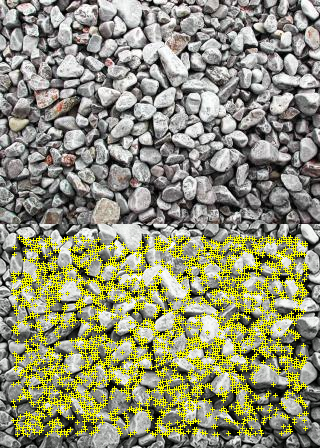
\includegraphics[width=2.5in]{pictures/vuforia_stones_comparison}
	\caption{Vuforia-Steine: Optimal trackbares Markerbild\newline (Quelle: Vuforia Developer Portal)}
	\label{vuforia_stones_image}
\end{figure}

\subsection{"`Hello-World"'-Anwendung}
Im Rahmen dieser Seminararbeit wurde eine "`Hello World"'-Anwendung für Android entwickelt, um ein Gefühl von der Funktionsweise des SDKs zu bekommen. Diese kann in Abbildung \ref{vuforia_sample} betrachtet werden. Hierbei wurde der in Abbildung \ref{vuforia_stones_image} zu sehende Marker verwendet. Sobald dieser von der Anwendung erfasst wird, werden die AR-Elemente projiziert. Wenn das Handy bewegt wird, bleibt der Roboter an der gleichen Stelle stehen. Wenn man den Marker bewegt, bewegt sich der Roboter mit diesem.\par
Für das initiale Erkennen des Markers ist aufgefallen, dass dieser zum Großteil von der Kamera erfasst sein muss. Anschließend kann sich jedoch ein Großteil auch außerhalb des Sichtfelds der Kamera befinden. Dies hat wahrscheinlich mit der hohen Feature-Anzahl des Bildes zu tun. Vermutlich dienen Gruppen von Features als Schlüssel zum Erkennen des Markers. Ein zweiter Marker mit weniger Features wird schwerer erkannt und darauf projizierte Objekte verschwinden schneller, sobald Teile des Markers verdeckt oder sich außerhalb des Bildes befinden.

\begin{figure}[h]
	\centering
	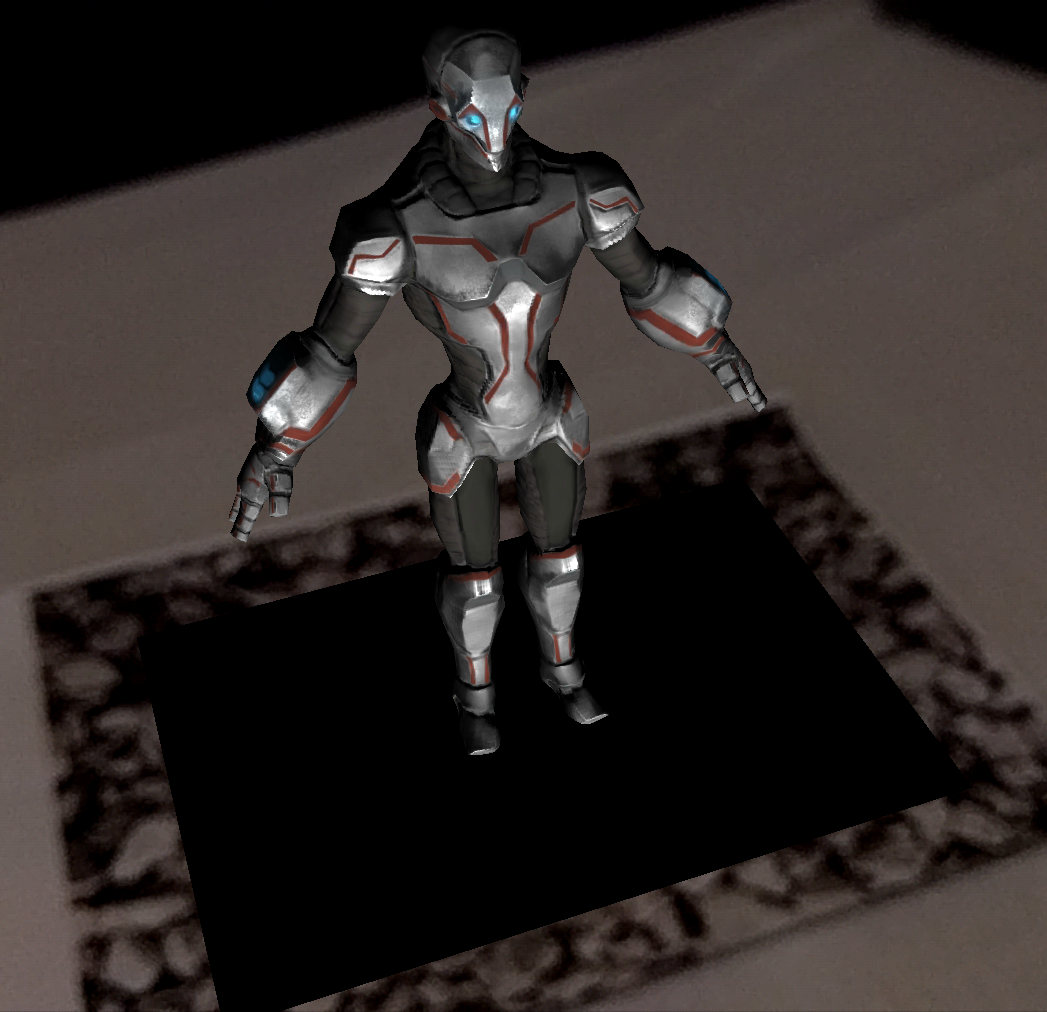
\includegraphics[width=2.5in]{pictures/vuforia_sample2}
	\caption{Auf dem Marker werden die AR-Elemente projiziert.\newline (Quelle: Autor)}
	\label{vuforia_sample}
\end{figure}

\subsection{ARToolKit}
Wenn man diese Schlüssel einzeln betrachtet, liegt der Vergleich mit dem ARToolKit \cite{artoolkit1}\cite{artoolkit2} nahe. Dabei werden ebenfalls Marker verwendet. Dort werden diese jedoch mit einem schwarzen Rahmen hervorgehoben und sollten nur einfache schwarze Muster enthalten. Das Bild der Kamera wird nach diesem Marker abgetastet. Sobald ein Marker gefunden wurde, wird seine Orientierung und Position anhand des gespeicherten Markers ermittelt. 3D-Objekte werden dann so projiziert, dass sie genauso ausgerichtet sind wie der Marker.\par
Nachteile sind hierbei, dass die Marker sehr simpel gehalten werden und immer vollständig sichtbar sein müssen. Ein sehr effizientes Beispiel hierfür ist zum Beispiel eine 3x3-Matrix, wobei jedes Feld entweder weiß oder schwarz ist. Daraus können sich dann mehrere Marker ableiten, die auch zusammen in einer Anwendung benutzt werden können. Hierbei ist noch zu beachten, dass jeder Marker einzigartig sein muss auch wenn er gedreht wird, d.h. ein weißes Feld in der oberen rechten Ecke der Matrix erzeugt den gleichen Marker wie ein weißes Feld in der unteren rechten Ecke, sofern der Rest schwarz ist.\par
Da Marker bei Vuforia nicht immer vollständig sichtbar sein müssen, scheint ein Marker also nicht nur \textbf{ein} Marker zu sein sondern besteht aus vielen einzelnen, welche sich aus den Features ergeben.

\subsection{Beispielanwendung}
Eine Android-App wurde an der Takming University of Science and Technology in Taipei zur Verbesserung des Lernens entwickelt\cite{vuforia_sample_application}. Diese wurde für diese Arbeit ausgewählt, da diese am besten dokumentiert ist und auch mehr Hintergründe von der Anwendung und Vuforia zeigt. Andere Apps, welche man z.B. über die Vufora-Webseite findet sind meist proprietär. Dazu zählen bspw. eine App von BMW, womit man ein Auto in seine Einfahrt projizieren kann und eine ähnliche App von Samsung für Fernseher im Wohnzimmer.\par
Bei dieser Applikation wurden Meereslebewesen auf die Marker projiziert, um diese besser analysieren zu können. Über ebenfalls projizierte Buttons können die Grafiken gewechselt werden. Das Aussehen und die Bewegungsmuster der Lebewesen soll den Studierenden so besser vermittelt werden können. Zusätzliche Informationen werden über eine Textbox unter der Figur dargestellt.
